\documentclass[border=7pt]{standalone}
\usepackage{amsmath}
\usepackage{tikz}
\usepackage{helvet}
\renewcommand{\familydefault}{\sfdefault}
\usetikzlibrary{arrows.meta,calc,positioning}

\definecolor{nullblue}{RGB}{220,234,245}
\definecolor{boundblue}{RGB}{70,130,180}
\definecolor{objectiveorange}{RGB}{224,138,20}
\definecolor{optred}{RGB}{184,54,54}
\definecolor{inkgray}{RGB}{70,70,70}

\begin{document}
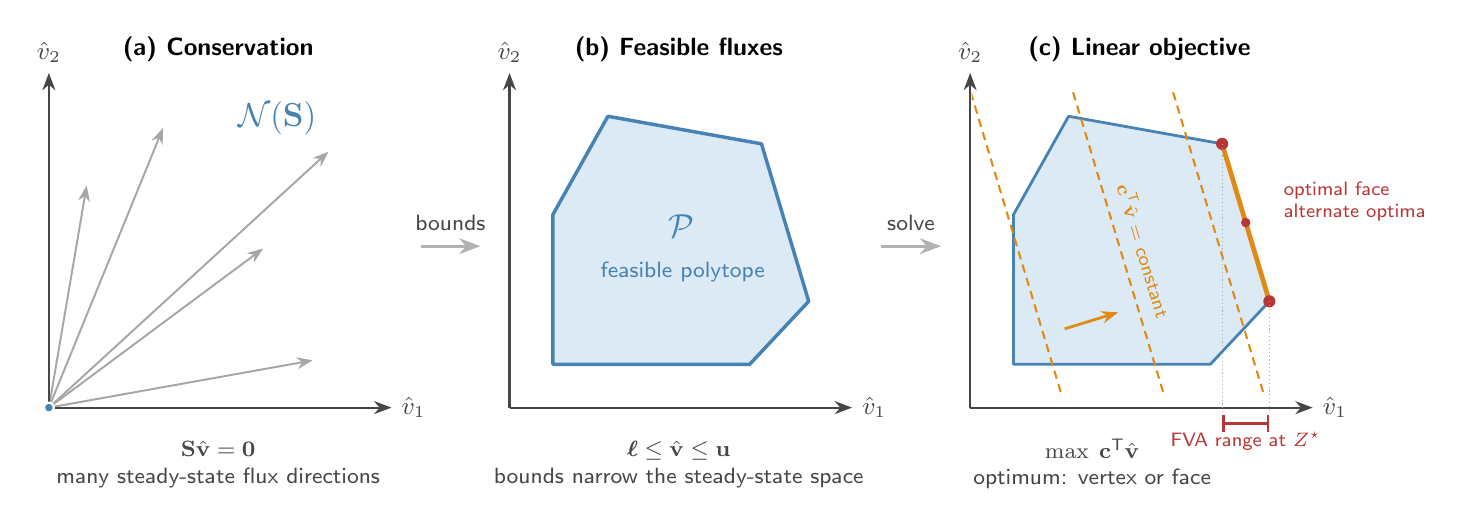
\begin{tikzpicture}[
  font=\small,
  axis/.style={-{Stealth[length=2.2mm]}, line width=0.75pt, inkgray},
  vector/.style={-{Stealth[length=2.0mm]}, line width=0.7pt, gray!70},
  contour/.style={line width=0.75pt, objectiveorange, densely dashed},
  stagearrow/.style={-{Stealth[length=2.7mm]}, line width=1.0pt, gray!60},
  paneltitle/.style={font=\bfseries\small, align=center},
  note/.style={font=\footnotesize, align=center, text=inkgray},
]

% Shared polygon coordinates in local panel coordinates.
\def\feasiblepolygon{(0.55,0.55)--(3.05,0.55)--(3.80,1.35)--(3.20,3.35)--(1.25,3.70)--(0.55,2.45)--cycle}

% -------------------------------------------------------------------------
% Panel A: a two-flux projection of the steady-state null space.
% -------------------------------------------------------------------------
\begin{scope}[shift={(0,0)}]
  \node[paneltitle] at (2.15,4.55) {(a) Conservation};
  % No filled region is drawn here: the entire open coordinate plane is the
  % displayed two-flux projection of the null space. Blue fill is reserved
  % for the bounded feasible polytope in panels (b) and (c).

  % Every candidate flux direction begins at the flux-space origin. Draw the
  % axes last so their baselines remain crisp where the vectors coincide.
  \coordinate (Oa) at (0,0);
  \draw[vector] (Oa) -- (3.35,0.60);
  \draw[vector] (Oa) -- (2.72,2.02);
  \draw[vector] (Oa) -- (1.45,3.55);
  \draw[vector] (Oa) -- (3.55,3.25);
  \draw[vector] (Oa) -- (0.48,2.82);
  \draw[axis] (0,0) -- (4.35,0) node[right] {$\hat v_1$};
  \draw[axis] (0,0) -- (0,4.25) node[above] {$\hat v_2$};
  \fill[white] (0,0) circle (2.2pt);
  \fill[boundblue] (0,0) circle (1.35pt);

  \node[font=\large, text=boundblue, fill=white, inner sep=2.5pt]
    at (2.90,3.67) {$\mathcal N(\mathbf S)$};
  \node[note] at (2.15,-0.72)
    {$\mathbf S\hat{\mathbf v}=\mathbf 0$\\
     many steady-state flux directions};
\end{scope}

\draw[stagearrow] (4.72,2.05) -- (5.48,2.05)
  node[midway,above=2pt,note] {bounds};

% -------------------------------------------------------------------------
% Panel B: bounds clip the null space to a convex feasible polytope.
% -------------------------------------------------------------------------
\begin{scope}[shift={(5.85,0)}]
  \node[paneltitle] at (2.15,4.55) {(b) Feasible fluxes};
  \draw[axis] (0,0) -- (4.35,0) node[right] {$\hat v_1$};
  \draw[axis] (0,0) -- (0,4.25) node[above] {$\hat v_2$};

  \fill[nullblue] \feasiblepolygon;
  \draw[boundblue, line width=1.25pt, line join=round] \feasiblepolygon;
  \node[font=\large, text=boundblue] at (2.18,2.30) {$\mathcal P$};
  \node[note, text=boundblue] at (2.20,1.72)
    {feasible polytope};

  \node[note] at (2.15,-0.72)
    {$\boldsymbol\ell\leq\hat{\mathbf v}\leq\mathbf u$\\
     bounds narrow the steady-state space};
\end{scope}

\draw[stagearrow] (10.57,2.05) -- (11.33,2.05)
  node[midway,above=2pt,note] {solve};

% -------------------------------------------------------------------------
% Panel C: objective contours support the polytope at an optimal face.
% -------------------------------------------------------------------------
\begin{scope}[shift={(11.70,0)}]
  \node[paneltitle] at (2.15,4.55) {(c) Linear objective};
  \draw[axis] (0,0) -- (4.35,0) node[right] {$\hat v_1$};
  \draw[axis] (0,0) -- (0,4.25) node[above] {$\hat v_2$};

  \fill[nullblue] \feasiblepolygon;
  \draw[boundblue, line width=1.0pt, line join=round] \feasiblepolygon;

  % Objective contours are parallel to the optimal edge from (3.80,1.35)
  % to (3.20,3.35). Moving them northeast increases c^T v.
  \begin{scope}
    \clip (0.02,0.02) rectangle (4.18,4.08);
    \draw[contour] (1.15,0.20) -- (0.00,4.03);
    \draw[contour] (2.45,0.20) -- (1.30,4.03);
    \draw[contour] (3.72,0.20) -- (2.57,4.03);
  \end{scope}
  \draw[objectiveorange, line width=1.7pt] (3.80,1.35) -- (3.20,3.35);
  \fill[optred] (3.80,1.35) circle (2.2pt);
  \fill[optred] (3.20,3.35) circle (2.2pt);
  \fill[optred] (3.50,2.35) circle (1.7pt);
  \node[font=\scriptsize, text=optred, align=left, anchor=west]
    at (3.86,2.62) {optimal face\\alternate optima};

  \draw[-{Stealth[length=2.1mm]}, objectiveorange, line width=1.0pt]
    (1.20,1.00) -- ++(0.68,0.21);
  \node[font=\scriptsize, text=objectiveorange, rotate=-73,
        fill=nullblue, inner sep=1.2pt]
    at (2.22,2.00) {$\mathbf c^{\mathsf T}\hat{\mathbf v}=\text{constant}$};

  % Projection of the optimal face onto reaction flux v1: an FVA range.
  \draw[gray!65, densely dotted] (3.20,3.35) -- (3.20,-0.05);
  \draw[gray!65, densely dotted] (3.80,1.35) -- (3.80,-0.05);
  \draw[{Bar[width=2.2mm]}-{Bar[width=2.2mm]}, optred, line width=0.9pt]
    (3.20,-0.20) -- (3.80,-0.20);
  \node[font=\scriptsize, text=optred] at (3.50,-0.43) {FVA range at $Z^\star$};

  \node[note] at (1.55,-0.72)
    {$\max\;\mathbf c^{\mathsf T}\hat{\mathbf v}$\\
     optimum: vertex or face};
\end{scope}

\end{tikzpicture}
\end{document}
